\section{Introducción}
\begin{frame}
\frametitle{Evolución de la Concurrencia en Java}

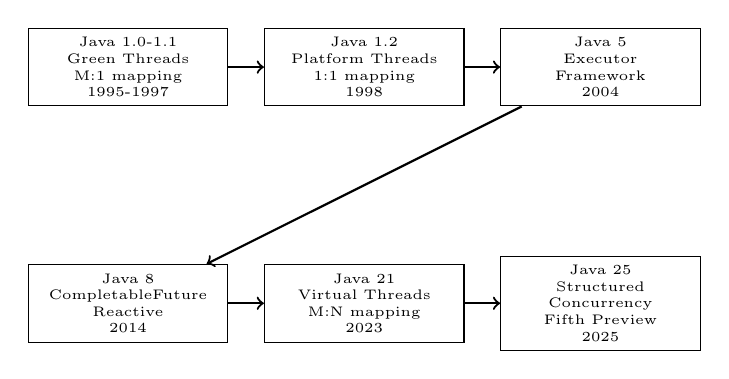
\begin{tikzpicture}[
     node distance=3cm,
    box/.style={draw, rectangle, text width=2.3cm, align=center,
                font=\tiny}
]
\node (green) [box] {Java 1.0-1.1\\Green Threads\\M:1 mapping\\1995-1997};
\node (platform) [box, right of=green] {Java 1.2\\Platform Threads\\1:1 mapping\\1998};
\node (executor) [box, right of=platform] {Java 5\\Executor\\Framework\\2004};
\node (reactive) [box, below of=green] {Java 8\\CompletableFuture\\Reactive\\2014};
\node (virtual) [box, right of=reactive] {Java 21\\Virtual Threads\\M:N mapping\\2023};
\node (structured) [box, right of=virtual] {Java 25\\Structured Concurrency\\Fifth Preview\\2025};

\draw [->, thick] (green) -- (platform);
\draw [->, thick] (platform) -- (executor);
\draw [->, thick] (executor) -- (reactive);
\draw [->, thick] (reactive) -- (virtual);
\draw [->, thick] (virtual) -- (structured);
\end{tikzpicture}

\vspace{1em}
\begin{alertblock}{Estado en Java 25}
\begin{itemize}
\item Virtual Threads: \textbf{Estable} (desde Java 21)
\item Scoped Values: \textbf{Estable}~\cite{JEP506}
\item Structured Concurrency: \textbf{Quinta Preview}~\cite{JEP505}
\end{itemize}
\end{alertblock}
\end{frame}
